% Material removed from Chapter 1 (author, 21 Nov 2026): the fishery example and its exercise.
% Replaced in Section 6 by the von Mises truss. Kept here for a later revision (not compiled).
% Figure: extra/st_fishery.pdf (made by the old block 5 of code/figures/fig_ch1.py, kept below).

\begin{example}[A fishery with a constant catch]\label{ex:st-fishery}
\index{harvesting model}%
Let $N(t)$ be the fish population of a lake, scaled so that the lake supports at
most $N = 1$. The fish reproduce logistically and are caught at the constant
rate $h$:
\begin{equation}\label{eq:st-fishery}
  \dot N = N(1 - N) - h .
\end{equation}
The steady states solve $N^2 - N + h = 0$, so
$N_\pm = \tfrac12\bigl(1 \pm \sqrt{1 - 4h}\bigr)$. The slope $f_N = 1 - 2N$ equals
$-\sqrt{1-4h}$ on $N_+$, the healthy stable stock, and $+\sqrt{1-4h}$ on $N_-$, an
unstable threshold: a stock pushed below $N_-$ collapses. Raising $h$ lowers the
parabola (Figure~\ref{fig:st-fishery}). At $h = \tfrac14$ the two roots meet at
$N = \tfrac12$, where $f_N = 0$, and for $h > \tfrac14$ no steady state is left.
This is a saddle-node.
\end{example}

\begin{figure}[ht]
  \centering
  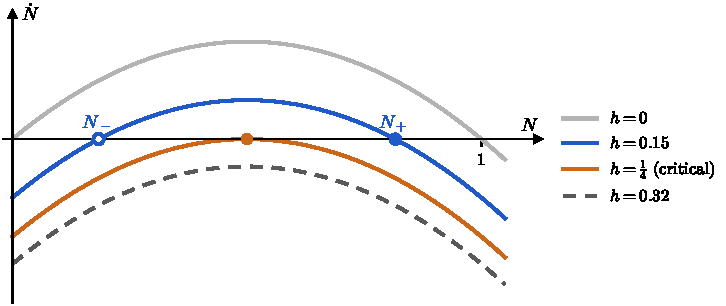
\includegraphics{ch01_bifurcation/figures/st_fishery.pdf}
  \caption{The fishery $\dot N = N(1-N) - h$. Increasing the catch $h$ lowers the
    parabola. The stable root $N_+$ and the unstable root $N_-$ merge at
    $h = \tfrac14$ and disappear.}
  \label{fig:st-fishery}
\end{figure}

The largest sustainable catch, $h = \tfrac14$, is also the edge of a cliff, and
the stock level gives little warning: at $h = 0.24$ the stock is still
$N_+ = 0.6$. The warning is in the recovery time
$\tau = 1/\sqrt{1 - 4h}$, which is $5$ time units at $h = 0.24$ and grows without
limit as $h \to \tfrac14$.
\draftnote{Keep the fishery in a mechanics book, or replace it by a snap-through
example (shallow arch) once Chapter 2 is written?}

\exercise{Maximum sustainable yield}\label{exo:st-fishery}
\index{harvesting model}%
For the fishery~\eqref{eq:st-fishery}:
(a)~derive $N_\pm$ and the critical catch $h = \tfrac14$;
(b)~a manager sets $h = 0.24$: find $N_+$ and $N_-$, and the largest sudden loss
of fish the stock survives;
(c)~explain why maximum sustainable yield is a dangerous target.
\begin{solution}
(a)~Example~\ref{ex:st-fishery}; $1 - 4h \ge 0$ requires $h \le \tfrac14$.
(b)~$\sqrt{1 - 0.96} = 0.2$, so $N_+ = 0.6$ and $N_- = 0.4$. A stock knocked below
$0.4$ collapses: the stock survives the loss of at most $0.2$, a third of it.
(c)~At $h = \tfrac14$ the two states merge: any disturbance, however small, or any
slight overestimate of $h_{\max}$, leads to collapse. The recovery time
$1/\sqrt{1-4h}$ is infinite there.
\end{solution}


% --- old figure code (block 5 of fig_ch1.py) ---
% # ----------------------------------------------- 5. fishery N' = N(1-N) - h
% fig, ax = plt.subplots(figsize=(W, 2.5))
% N = np.linspace(0, 1.05, 200)
% for h, col, ls, lab in [(0.0, (0.7, 0.7, 0.7), "-", r"$h=0$"),
%                         (0.15, CU, "-", r"$h=0.15$"),
%                         (0.25, ORANGE, "-", r"$h=\frac{1}{4}$ (critical)"),
%                         (0.32, (0.35, 0.35, 0.35), (0, (4, 3)), r"$h=0.32$")]:
%     ax.plot(N, N * (1 - N) - h, color=col, ls=ls, lw=1.5, label=lab)
% middle_axes(ax)
% Np, Nm = (1 + np.sqrt(0.4)) / 2, (1 - np.sqrt(0.4)) / 2
% ax.plot(Np, 0, "o", color=CU, ms=5, zorder=5)
% ax.plot(Nm, 0, "o", mfc="white", mec=CU, mew=1.4, ms=5, zorder=5)
% ax.plot(0.5, 0, "o", color=ORANGE, ms=4.5, zorder=5)
% ax.text(Np, 0.025, r"$N_+$", color=CU, ha="center")
% ax.text(Nm, 0.025, r"$N_-$", color=CU, ha="center")
% ax.set_xticks([1]); ax.set_yticks([])
% ax.set_xlim(-0.02, 1.12); ax.set_ylim(-0.42, 0.32)
% ax.text(1.12, 0.015, r"$N$", ha="right"); ax.text(0.02, 0.30, r"$\dot N$")
% ax.legend(loc="center left", bbox_to_anchor=(1.02, 0.5), frameon=False)
% save(fig, "st_fishery.pdf")
% 
